% Chapter 4: Design and Implementation

\chapter{Descripción informática} % Main chapter title

\label{Chapter4} % Reference

%-------------------------------------------------------------------------------

En este capítulo se describe el desarrollo completo del proyecto, desde el diseño hasta la implementación de este, así como la metodología utilizada para la correcta evolución de este.

\section{Diseño}
Para la realización del desarrollo del proyecto se ha optado por seguir un paradigma de programación orientada a objetos y se ha planteado la arquitectura que se muestra en el diagrama de clases de la figura \ref{fig:diagrama-clases}.
La implementación parte de un documento principal, en este caso se trata de un script ejecutable, grasp\_main.py, que contiene la información inicial y las llamadas a las clases y métodos de estas, necesarios para obtener los resultados al problema.

A continuación de este parten las clases:
 \begin{itemize}
	\item \textbf{Instance}: Esta clase contendrá toda la información relacionada con una instancia o definición de grafo del problema, la cuál se compone de la clase \textbf{Node}, que contiene toda la información relativa a un nodo, así como operaciones relacionadas con el mismo.
	\item \textbf{SolutionGrasp}: Esta clase contendrá los métodos necesarios para la implementación del algoritmo \gls{GRASP} y de la búsqueda local.
	\item \textbf{GraphUtils}: Esta clase está formada por métodos estáticos en su mayoría, y contendrá todos los métodos de utilidad relacionadas con los grafos, así como la posterior exportación a fichero de los resultados obtenidos durante el proceso. También se compone de la clase \textbf{Logger}, la cuál ayuda a configurar el sistema de registros del proyecto, con el que trazar errores y ver el estado del progreso más fácilmente.
\end{itemize}

También se encuentran las clases:
 \begin{itemize}
	\item \textbf{SolutionGreedy}: Esta clase abstracta contiene lo necesario para construir una solución completa mediante un algoritmo voraz. La definición completa se refiere a los atributos density, el cuál indica la densidad del grafo del que parte el proceso; clique, que contiene el listado de nodos que forman parte de la solución; sol\_value, el cuál indica el valor de la solución o función objetivo; cardinality, que contiene el valor del número de nodos de la solución y compute\_time, que indica el tiempo total de computo en hallar esa solución.
	\item \textbf{SolutionGreedyRatio}: Clase especializada en la obtención del mejor candidato posible por la condición de ratio.
	\item \textbf{SolutionGreedyNeighbors}: Al igual que \textbf{SolutionGreedyRatio}, esta clase se especializa en encontrar el mejor nodo candidato, en este caso, con mayor número de nodos vecinos.
\end{itemize}


\begin{figure}[H]
	\centering
	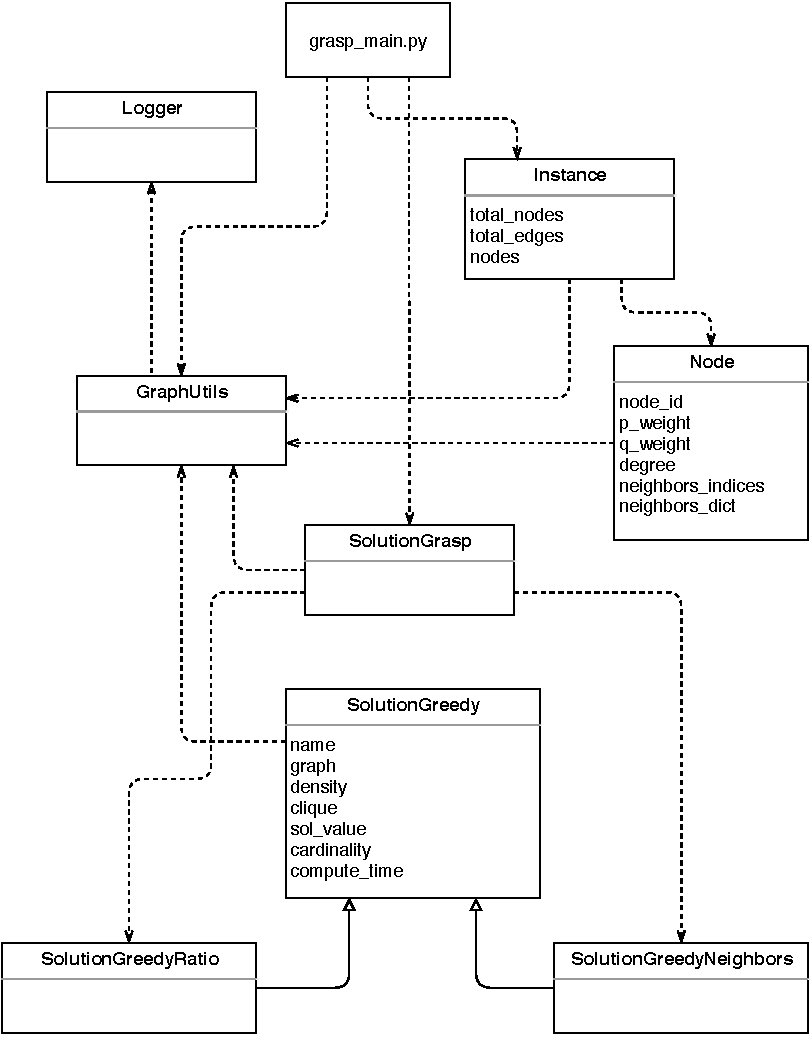
\includegraphics{Figures/Diagrama-clases.pdf}
	\caption{Diagrama de clases del proyecto.}
	\label{fig:diagrama-clases}
\end{figure}

\section{Implementación}
\label{sec:implementacion}
La implementación de este proyecto se basa en la ejecución de un script\footnote{Secuencia de ordenes o instrucciones que serán interpretadas para su ejecución.}, escrito en lenguaje Python, que parte de una clase principal caracterizada por contener la siguiente sentencia de código:
 \begin{lstlisting}[language=Python]
 if__name__ == "__main__"
 \end{lstlisting}
 Dicha sentencia posibilita la ejecución del script mediante el comando:
  \begin{lstlisting}[language=bash]
  python grasp_main.py
 \end{lstlisting} 

 Este script, en adelante Grasp Main, tiene la configuración necesaria para ajustar los parámetros del programa:
 \begin{itemize}
 	\item Número de iteraciones a realizar por cada fichero.
 	\item Ruta donde se encuentran los ficheros de definición de los grafos a procesar o instancias.
 	\item Ruta de los ficheros de resultados generados por el programa.	
 	\item Valores de $\alpha$ para ajustar la aleatoriedad del algoritmo.
 \end{itemize}

Grasp Main se encarga de recorrer recursivamente los ficheros que se encuentren en la ruta de recursos definida y, por cada uno de los ficheros encontrados, crea un objeto de tipo Instance, añadiendo la siguiente información del grafo:
 \begin{itemize}
	\item Número de nodos.
	\item Número de aristas.
	\item Estructura de datos con los nodos del grafo.
\end{itemize}

Esta estructura de datos contiene tantos objetos de tipo Node como tenga el grafo, cada uno de ellos con la siguiente información:
 \begin{itemize}
	\item Identificador del nodo.
	\item Valor del peso p.
	\item Valor de peso q.
	\item Grado del nodo.
	\item Estructura de datos con las relaciones de este nodo con otros nodos del grafo.
\end{itemize}

Tras terminar esta operación se realiza el procesado un número N de veces, según se haya definido previamente en la configuración de la aplicación, y por cada tipo de constructivo, los cuales serán explicados más adelante.

A partir de este punto se invoca la función $find\_grasp\_solution$ disponible en la clase SolutionGrasp y que implementa al algoritmo \gls{GRASP} anteriormente descrito. Esta función inicializa los siguientes datos:
\begin{itemize}
	\item vertex, el cuál es obtenido de manera aleatoria entre todos los nodos del grafo.
	\item solution, conjunto inicializado con el vértice obtenido anteriormente.
	\item cl, lista de candidatos posibles para encontrar una solución.
\end{itemize}

Para la fase constructiva del algoritmo, la implementación se apoya en la función $get\_g$ que obtiene un listado de posibles candidatos. Según el tipo elegido en la configuración inicial, se creará un objeto del constructivo específico, SolutionGreedyRatio o SolutionGreedyAdjacent. Estos heredan de la clase abstracta\footnote{En programación orientada a objetos, es un tipo de clase que no puede ser instanciada, y por lo general sirve para definir otras clases de este tipo.} SolutionGreedy, la cual tiene la información compartida por ambos tipos, y delega la implementación de la función $find\_better$ en cada una de las clases específicas, quienes mediante un algoritmo de tipo voraz buscan una solución factible en un tiempo muy reducido.

Una vez se obtiene el listado de candidatos, es procesado mediante la función $get\_rcl$, la cual haciendo uso del valor de $\mu$, calculado como se mostró en el algoritmo \ref{alg:grasp} con el valor de $\alpha$, permite obtener la lista de candidatos restringida denominada en el algoritmo como $RCL$. A partir de este momento el siguiente paso es escoger de manera aleatoria un nodo de esta lista e incluirlo en el conjunto solución, eliminando de la lista $CL$ los nodos que no son adyacentes a este, ya que no formarían una solución factible. Esta operación es realizada hasta que la lista de candidatos esté vacía.

Obtenida esta solución preliminar, se aplica la búsqueda local para la mejora de la misma, mediante la función $apply\_ls$. En esta función en primer lugar se obtienen los vecinos de los nodos que forman parte de la solución y son ordenados de mayor a menor ratio. Cada nodo es añadido a la solución previa, comprobando si forma o no una nueva solución factible. Si no cumple con las restricciones, se eliminarán todos los nodos mediante una función de exclusión de nodos. Esta elimina todos los nodos que impiden que se forme solución. Una vez cumple con las restricciones, se añaden todos los nodos adyacentes con el fin de obtener un clique máximo.Esta solución parcial es añadida a un listado de la que se seleccionará la mejor opción una vez finalizado el procesamiento de todos los nodos.

Para mantener el código ordenado se ha implementado la clase GraphUtils, la cual contiene información necesaria y métodos útiles para el procesado de las instancias, así como la exportación a ficheros de tipo CSV\footnote{Es un tipo de ficheros de texto simple en el que se almacenan datos separados en columnas por comas o por punto y coma, y las filas por salto de línea.} de los resultados obtenidos.

Con el fin de probar las diferentes funciones del proyecto se han escrito casos de prueba mediante la librería de Python unittest\footnote{https://docs.python.org/3/library/unittest.html}.

\section{Metodología empleada}
Para el desarrollo de este proyecto se ha optado por seguir una metodología de tipo iterativa e incremental, la cual permite evolucionar el proyecto progresivamente e ir adaptándose a los requisitos del cliente, en este caso los tutores del proyecto, en el menor tiempo posible, mejorando así la calidad del producto final con el menor esfuerzo.

Estas iteraciones e incrementos de funcionalidad se han realizado durante todo el desarrollo del proyecto, mediante reuniones, con un lapso de aproximadamente 3 o 4 semanas entre ellas, corrigiendo errores de la iteración anterior si los hubiera y aumentando la funcionalidad del producto a entregar, de esta manera se consigue una evolución progresiva y segura de los requerimientos que el proyecto exige.

Para mantener el control y administrar las tareas a realizar, las que se están desarrollando y las que han finalizado, se ha usado el administrador de proyectos Trello\footnote{https://trello.com/es} el cual mediante tarjetas permite conocer las tareas del proyecto, así como su estado, detalles de esta y añadir nuevas si fuera necesario. En la figura \ref{fig:trello-tarjetas} se muestra un ejemplo de uso del sistema de tarjetas que ofrece la herramienta.

\begin{figure}[H]
	\centering
	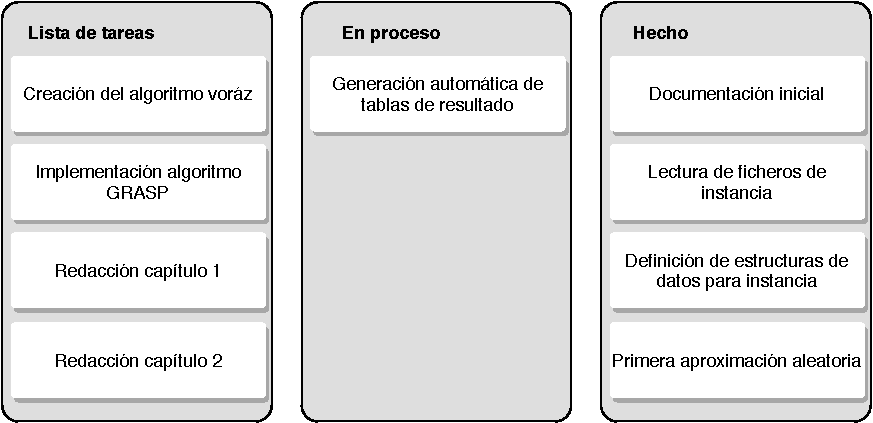
\includegraphics{Figures/trello-tarjetas.pdf}
	\caption{Ejemplo del sistema de tarjetas de Trello.}
	\label{fig:trello-tarjetas}
\end{figure}

En cuanto al mantenimiento de versiones del proyecto, se ha usado el sistema de control de versiones Git\footnote{https://git-scm.com/} y gestionado a su vez a través del portal de alojamiento remoto de repositorios GitHub\footnote{https://github.com/}. Para interactuar entre el repositorio local y el repositorio remoto se ha optado por hacer uso tanto de la terminal, mediante los comandos del propio sistema de control de versiones Git, como del cliente para tal propósito GitKraken\footnote{https://www.gitkraken.com/} el cual permite, mediante su sencilla e intuitiva interfaz, un control exhaustivo sobre las ramas y versionado de las distintas piezas de código del proyecto en el que se trabaja, así como revisar posibles conflictos que se produzcan.
%-------------------------------------------------------------------------------

